\newpage
\chapter{Proyecto técnico}

\section{Análisis del problema}

    \subsection*{Definición y características clínicas del queratocono}

        El queratocono es una enfermedad ocular en la que la córnea (la parte transparente y curva en la superficie del ojo) se debilita y adelgaza progresivamente, deformándose hasta tomar una forma cónica en lugar de su curvatura normal (Figura~\ref{fig:comparacion_corneas}). Esto altera la manera en que la luz ingresa al ojo, generando visión borrosa y distorsionada que empeora con el tiempo si no se detecta en etapas iniciales \citeA{queratocono}.

        \vspace{-0.5 cm}
        \begin{figure}[H] \centering
            \begin{subfigure}[b]{0.45\textwidth} \centering
                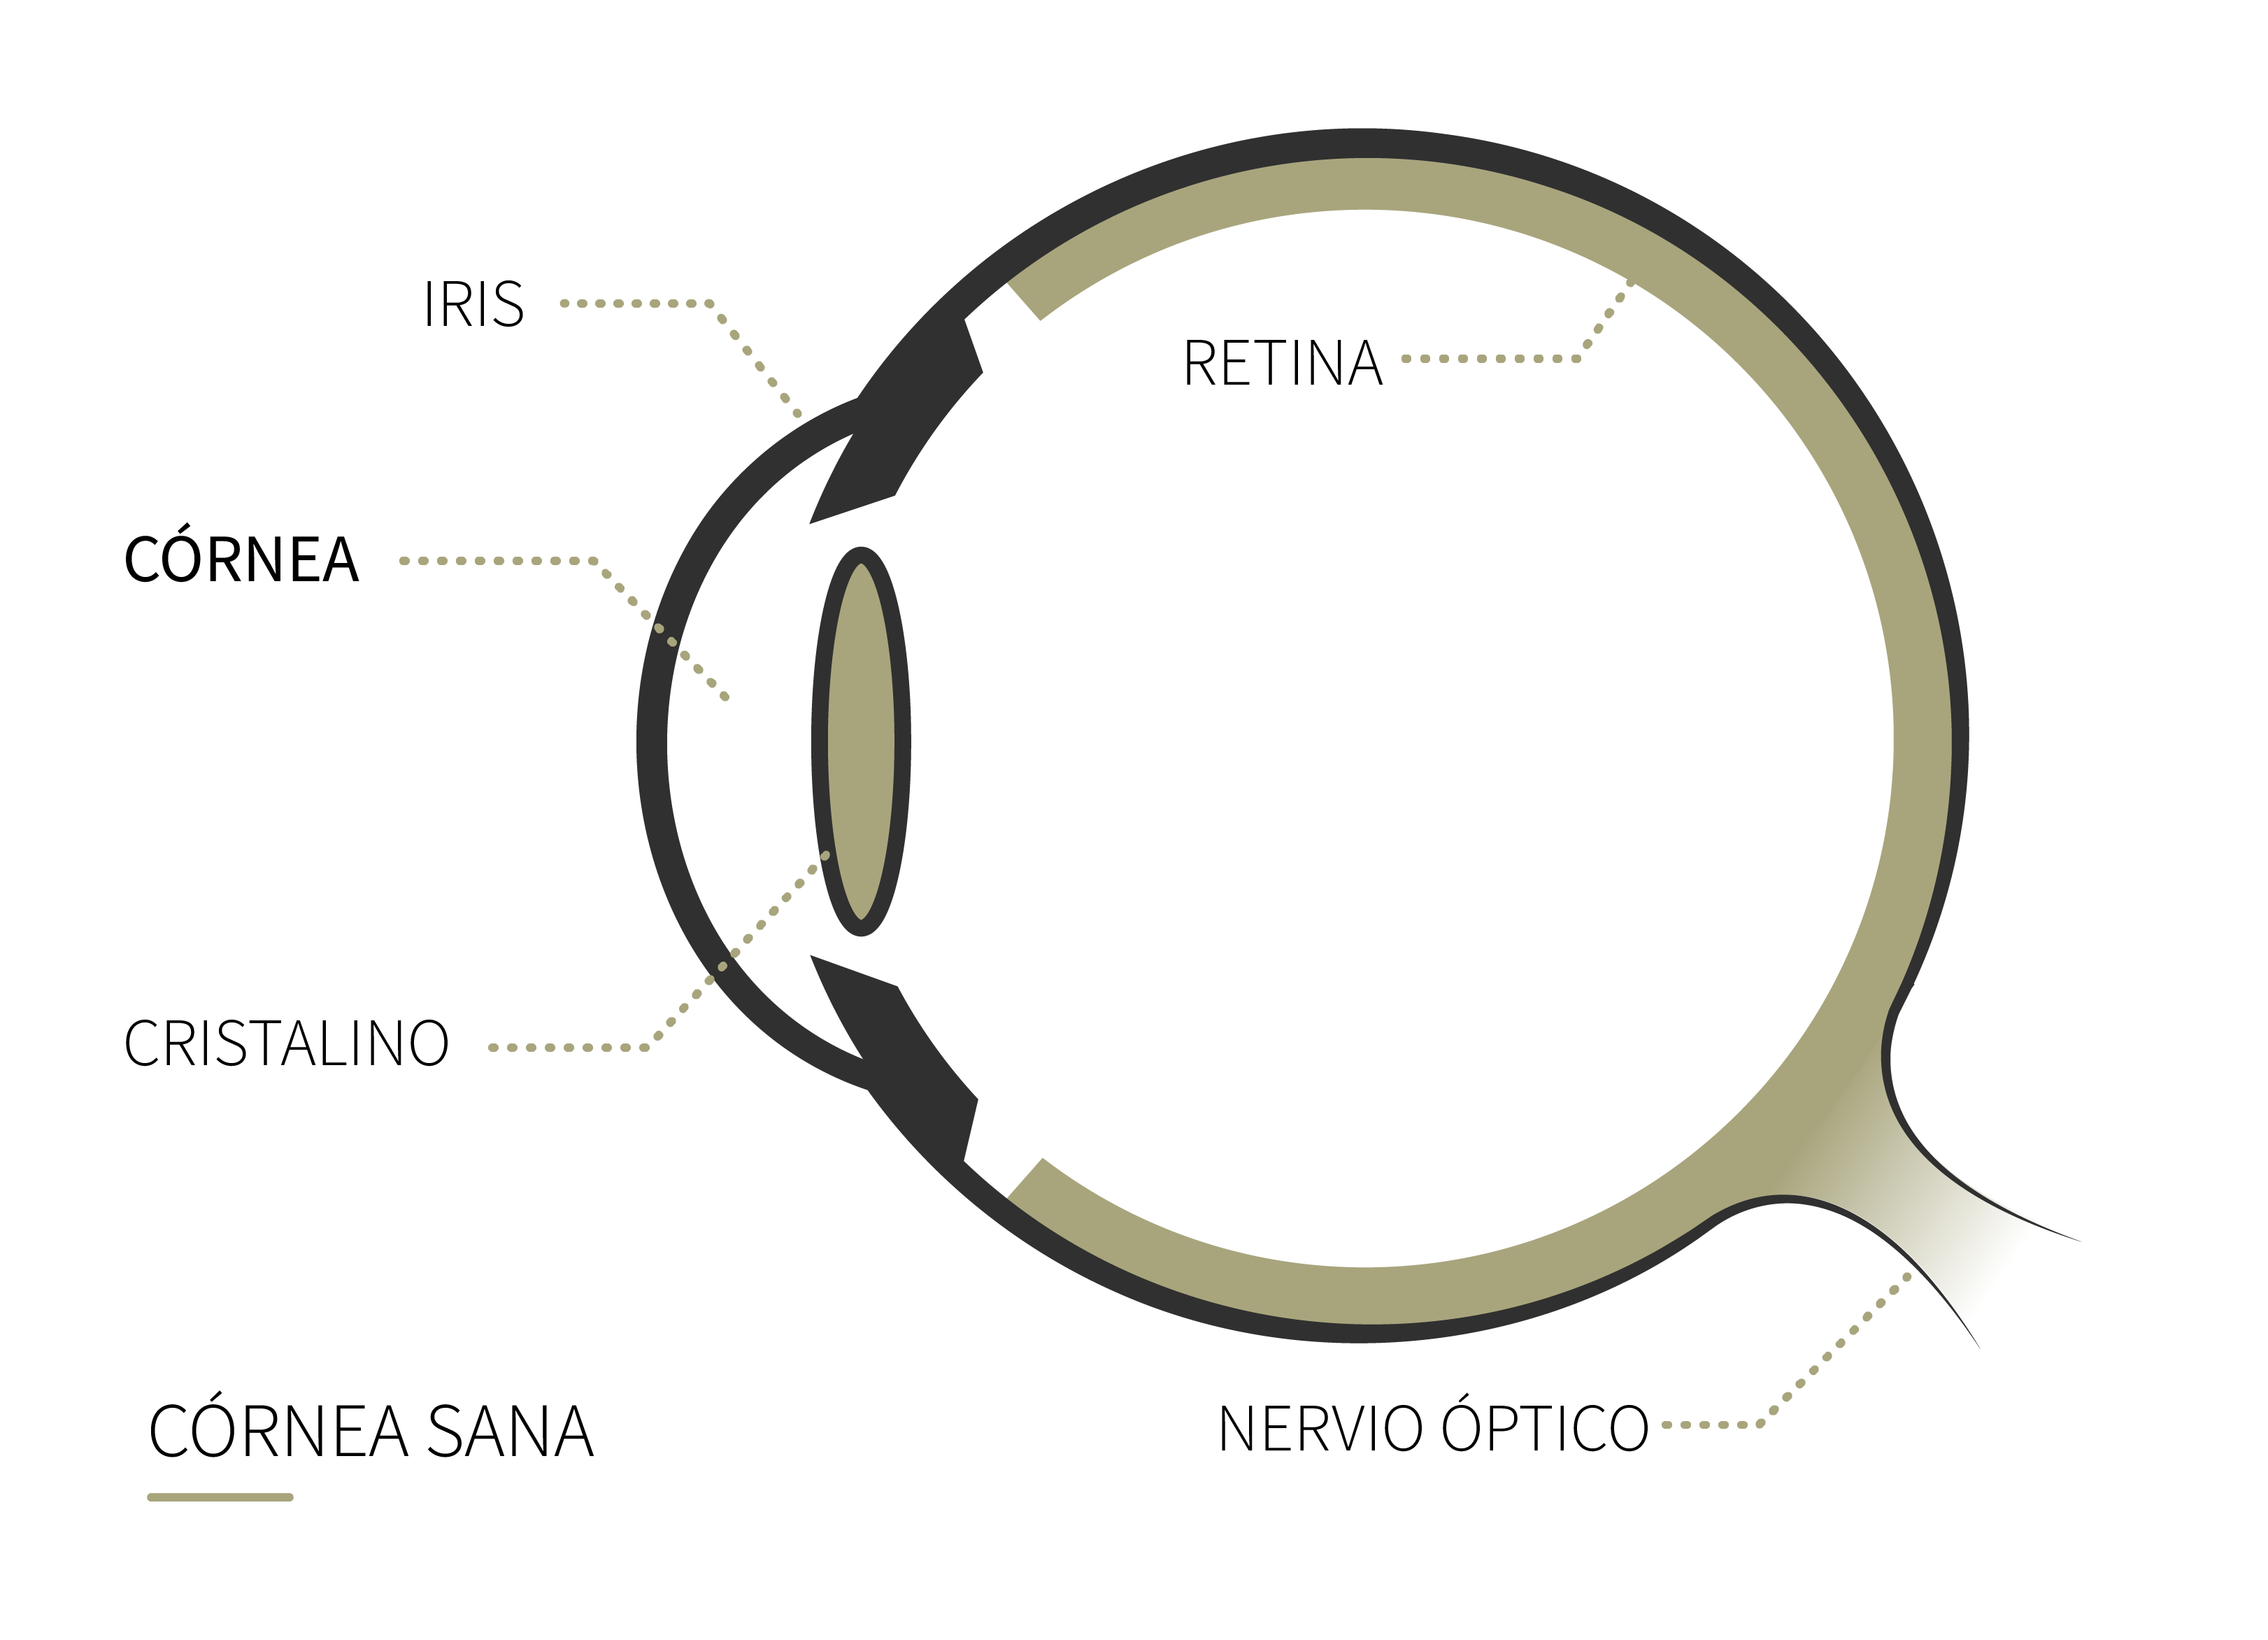
\includegraphics[width=\textwidth]{img/queratocono_deformacion_a.png} 
                \caption{Córnea sana}
                \label{fig:cornea_a}
            \end{subfigure}
            \hspace{-1 cm}
            \begin{subfigure}[b]{0.45\textwidth} \centering
                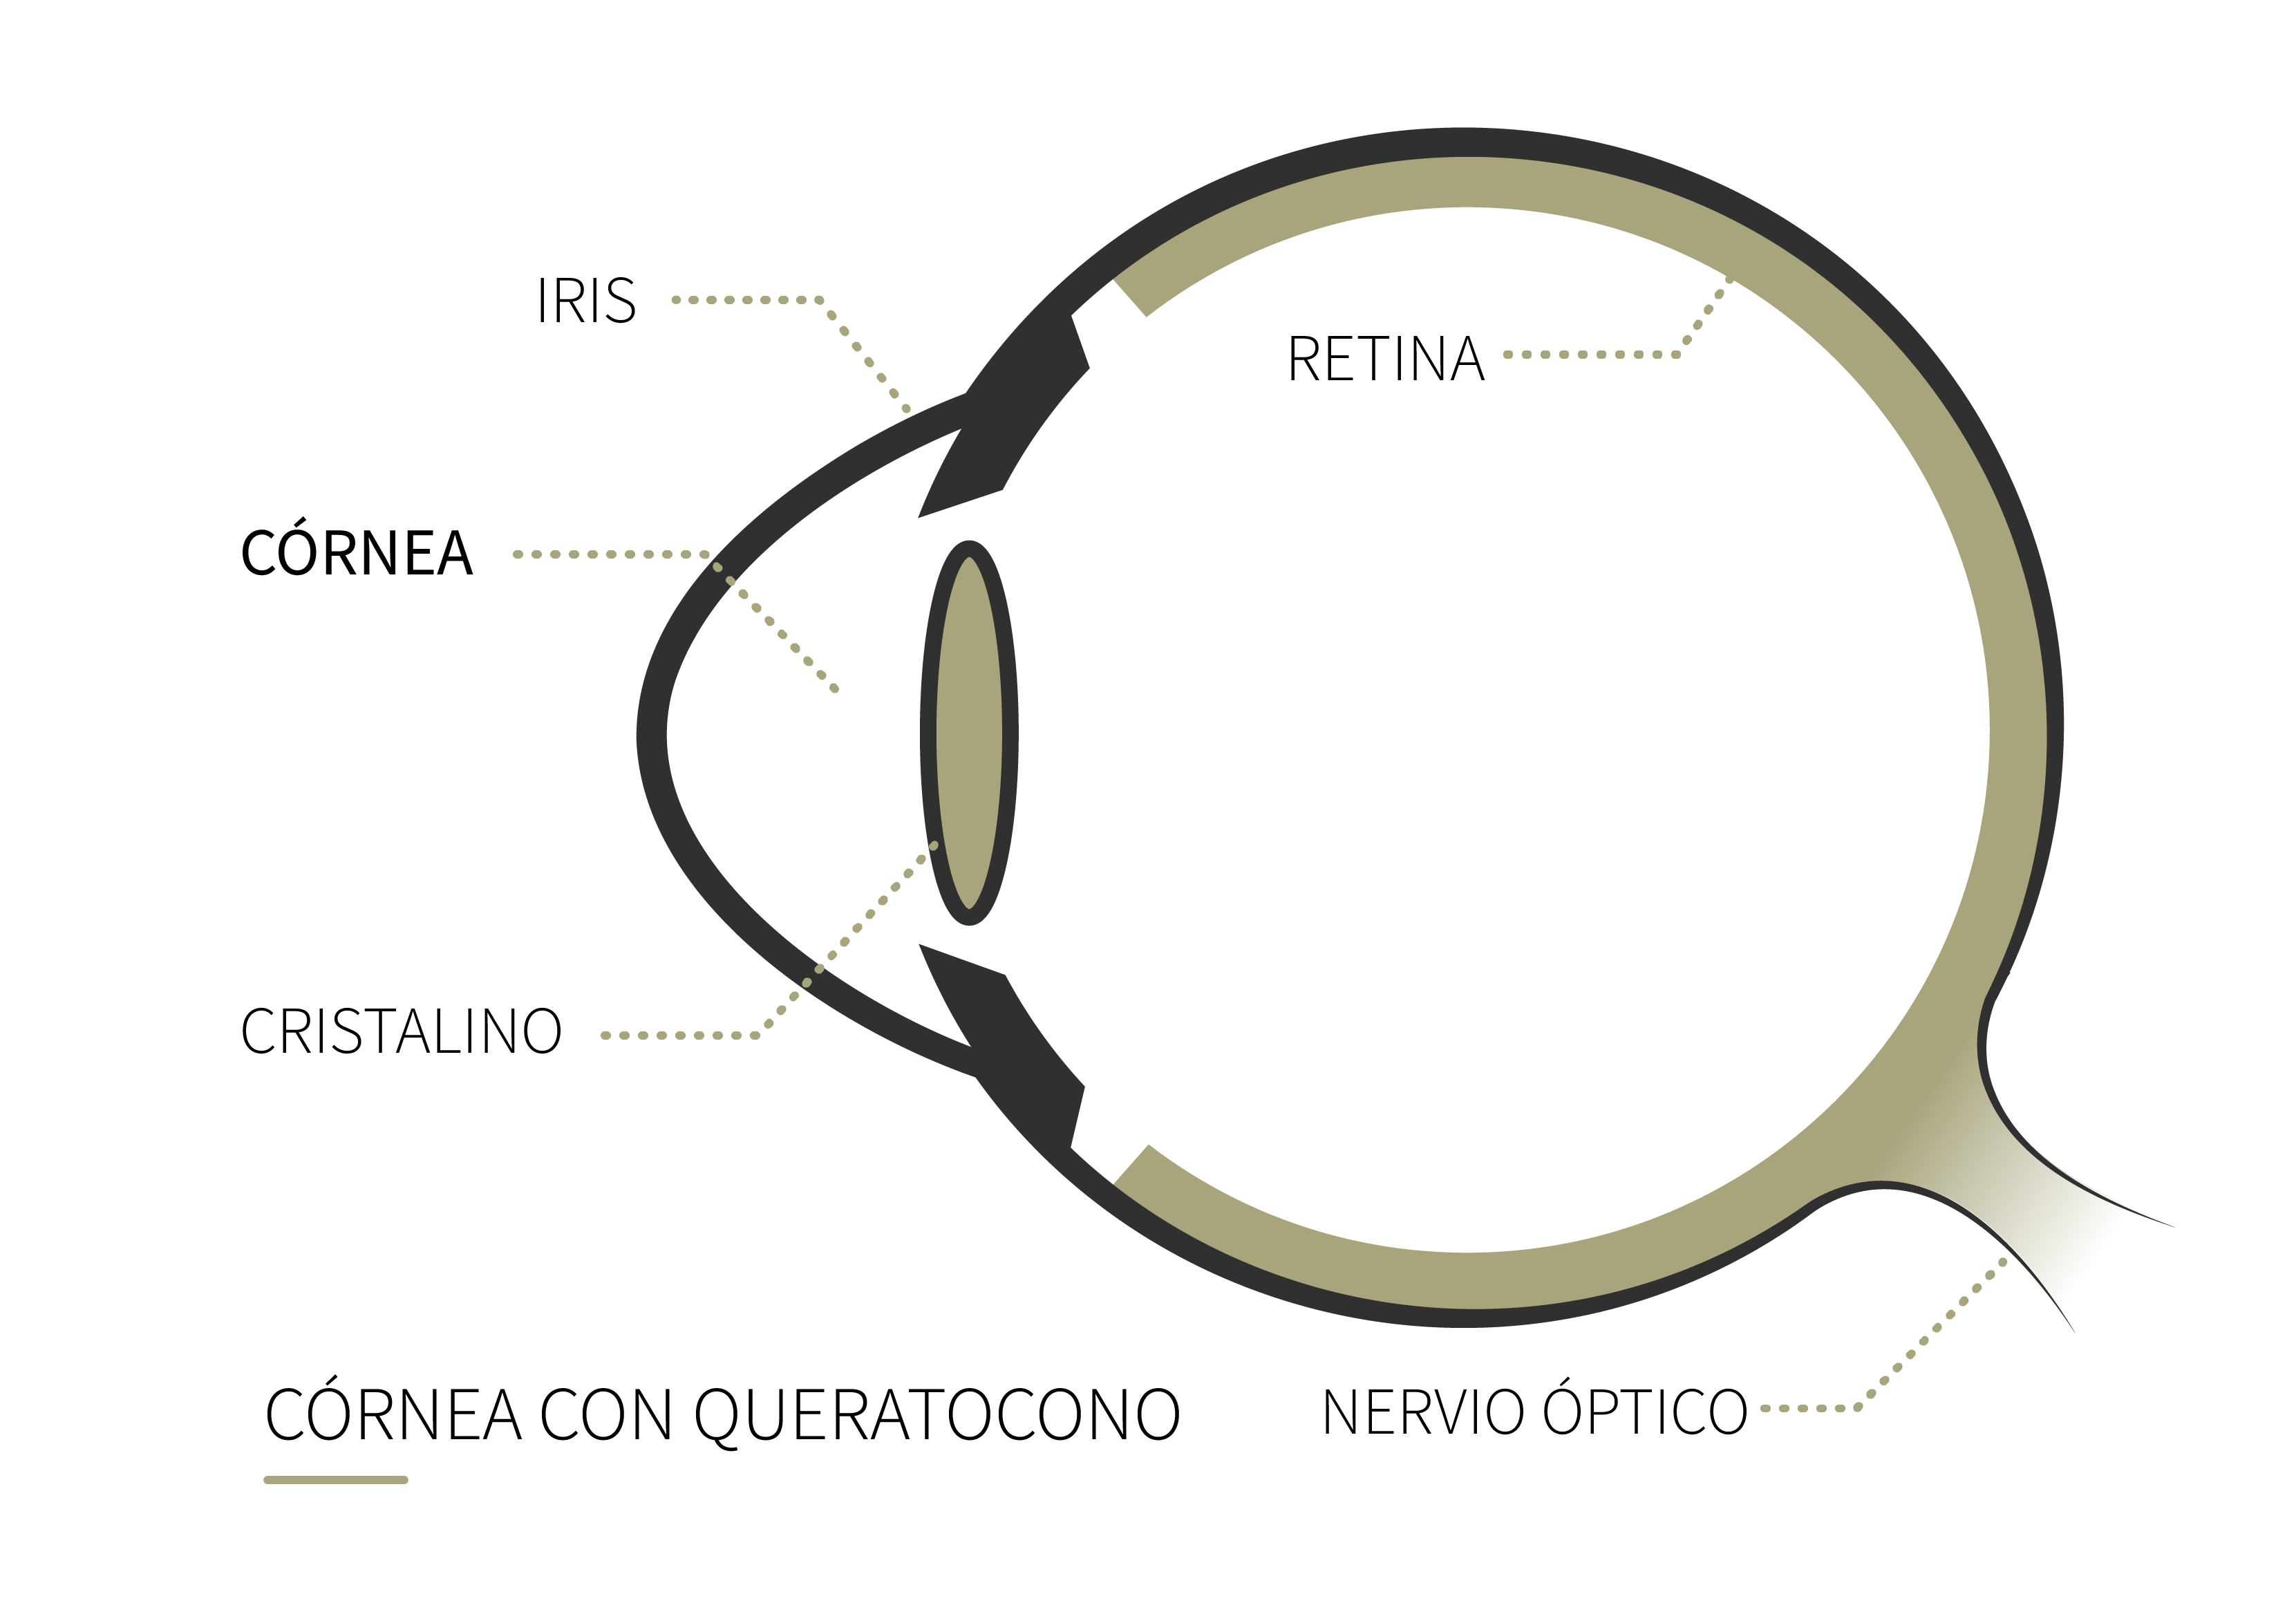
\includegraphics[width=\textwidth]{img/queratocono_deformacion_b.png}
                \caption{Córnea con queratocono}
                \label{fig:cornea_b}
            \end{subfigure}
            \caption{Comparación anatómica entre córnea sana y córnea con queratocono.}
            \label{fig:comparacion_corneas}
        \end{figure}

    \par\vspace{-0.5 cm}
    \subsection*{El desafío del diagnóstico temprano}
    
        El queratocono presenta la dificultad de que sus manifestaciones iniciales son sutiles y pueden confundirse con miopía o astigmatismo común. Esta interpretación está condicionada por la experiencia del profesional, lo que aumenta la probabilidad de errores, especialmente en etapas subclínicas donde la patología se manifiesta de forma discreta y no resulta evidente en una revisión superficial del estudio.
    
        Esta situación se ve agravada por la rápida aparición y avance de la enfermedad en edades tempranas de los pacientes, lo que representa un punto crítico en cuanto al tiempo de diagnóstico y tratamiento. La demora en la detección puede derivar en una progresión irreversible del daño corneal, llegando en estancias medias y avanzadas a necesitar intervención quirúrgica para no perder la visión \citeA{deteccion_temprana}.
        
        La interpretación visual de mapas topográficos y tomográficos puede derivar en diagnósticos confusos o tardíos, particularmente en manos de médicos con menos experiencia, lo que fundamenta la necesidad de generar herramientas de asistencia al diagnóstico basadas en Inteligencia Artificial (IA) para estandarizar los criterios de evaluación y reducir la variabilidad inherente al proceso \citeA{queratocono_ia}.

    \subsection*{Indicadores cuantitativos}

        Se estima que afecta a más de $23,7$ millones de personas a nivel mundial, con una prevalencia global de $289$ casos por cada $100.000$ habitantes~\citeA{prevalencia_kc}. A pesar de los avances en imagenología corneal, la detección de estadios subclínicos es un desafío dado que los sistemas de IA alcanzan una sensibilidad del $90\%$ en estos casos, frente al $98,6\%$ en casos ya manifiestos, es decir que uno de cada diez ojos con queratocono subclínico pasa desapercibido, contra menos de dos de cada cien con deformación mas avanzada~\citeA{sensibilidad_ia_subclinica}.
        
        Esta dificultad se traduce en demoras diagnósticas de hasta $2,9$ años entre la primera consulta optométrica y la derivación oftalmológica~\citeA{demora_diagnostica}, retraso que resulta crítico considerando que hasta el $88\%$ de los casos de ectasia corneal post-quirúrgica\footnote{Adelgazamiento y encurvamiento progresivo de la córnea posterior a una cirugía refractiva, cuando el tejido remanente pierde la resistencia necesaria para sostener la presión intraocular. Puede llegar a requerir un trasplante.} se atribuyen a ojos queratocónicos que no fueron detectados a tiempo~\citeA{falsos_negativos_ectasia}.

    \subsection*{Impacto local}
    
        En la provincia de Misiones, se ha reportado un aumento de casos de queratocono en la ciudad de Oberá~\citeA{misiones}. El problema real es que la infraestructura diagnostica se concentra en Posadas y Alem donde, para un paciente de zonas remotas de la provincia, una consulta podría ser su única oportunidad de detección dados los costos de traslado. Lo que evidencia la relevancia regional de la problemática. 
        
        Un soporte a la decisión clínica actuaría como una herramienta de ayuda para referenciar los criterios de evaluación, pudiendo reducir el riesgo de errores diagnósticos y permitiendo intervenciones oportunas para preservar la visión de los pacientes.
        
    \subsection*{Riesgos de implementación y barreras normativas}
    
        Al tratarse de una aplicación en el ámbito de la salud, la implementación de este sistema conlleva riesgos críticos que deben ser tenidos en cuenta. La integración de modelos de IA exige una rigurosa validación externa o local. Este proceso es fundamental para contrastar el rendimiento del algoritmo con la realidad clínica diaria, permitiendo evaluar y documentar de manera rigurosa la fiabilidad y eficacia del sistema bajo las condiciones y recursos de nuestra región.
    
        Por otro lado, la Disposición ANMAT 9688/19 establece en su artículo 26 que todo \textit{software} que se encuadre en la definición de producto médico debe inscribirse en el Registro de Productores y Productos de Tecnología Médica~\cite{dispo_9688}, requisito que alcanza directamente a este sistema. La inscripción no certifica por sí sola que el producto sea seguro, si no que exige presentar los ensayos que respaldan el informe de Requisitos Esenciales de Seguridad y Eficacia, con una profundidad que depende de la clase de riesgo asignada según la Disposición 2318/02~\cite{dispo_2318}.
        
        La responsabilidad legal de los datos locales recae en los oftalmólogos consultados, en su labor de anonimizar los estudios provistos. Por otro lado, los datos presentes en los \textit{datasets} internacionales~\citeA{kaggle,zenodo,insight} ya vienen anonimizados previamente para su uso, garantizando la transparencia y validación clínica según las normativas de protección de datos personales~\citeA{ley_25326}.

\phantomsection
\par\vspace{-0.2 cm}
\section{Antecedentes}

    \par\vspace{-0.25 cm}
    \subsection*{Redes neuronales recurrentes (RNN)}

        Un antecedente fundamental es el modelo de aprendizaje profundo multimodal presentado por Shafi Balal en el congreso ESCRS 2025, abordando la problemática de que los médicos no pueden predecir con certeza qué pacientes progresan hacia estadios graves y cuáles son estables, saturando los servicios con seguimientos frecuentes. Su sistema utiliza redes neuronales recurrentes para analizar datos de sólo dos visitas, logrando clasificar a los pacientes en grupos de bajo o alto riesgo de progresión a dos años~\citeA{shafi_balal}.

        Este trabajo demuestra dos cosas: es posible construir modelos predictivos con una cantidad reducida de información clínica y que es viable estratificar el riesgo de progresión. Esto es relevante puesto que valida uno de los fines del trabajo propuesto, la estratificación. Además, verifica que no precisamos de un banco de datos de validación extenso con muestras locales.

    \par\vspace{-0.1 cm}
    \subsection*{Redes neuronales convolucionales (CNN)}
    
        Por otro lado, el desarrollo del algoritmo KeratoDetect se enfoca en la dificultad de detectar el queratocono en etapas subclínicas. Este algoritmo demostró que los modelos basados en redes neuronales convolucionales pueden identificar patrones patológicos que el ojo humano podría omitir, procesando imágenes corneales para una clasificación binaria con alta precisión~\citeA{kerato_detect}.

        Este antecedente se centra exclusivamente en la detección, sin abordar la estratificación ni integración a sistemas para oftalmólogos. Esto nos sirve para validar que es posible el otro punto objetivo del trabajo, la detección. Además, justifica la utilización de redes CNN para definir la arquitectura de procesamiento.

    \par\vspace{-0.1 cm}
    \subsection*{Herramientas médicas e investigación}
    
        En el ámbito local, no existen competidores directos con un software como producto médico específico para queratocono en Argentina. El referente más cercano es Entelai~\citeA{entelai}, una \textit{startup} líder en el país en la aplicación de IA para el análisis de imágenes médicas, cuyo modelo de validación asistida permite a los médicos procesar informes con rapidez. A nivel internacional, proyectos como KERAFound y el sistema multi-agente AEYE~\citeA{aeye} están evolucionando desde la investigación académica hacia las herramientas comerciales de aplicación.
    
        Mediante estos antecedentes se demuestra que es posible predecir de la enfermedad y estratificar su riesgo basándose en imágenes topográficas y datos clínicos relevantes. Además, la industria está interesada en la adopción de aplicaciones médicas para el apoyo en el flujo de trabajo e investigar estas herramientas.

    \subsection*{\textit{Vision Transformers}}

        En paralelo al uso de arquitecturas convolucionales, distintos trabajos recientes han incorporado \textit{Vision Transformers} (VT) para el análisis de queratocono, superando las limitaciones de las CNN en la captura de dependencias espaciales de largo alcance dentro de la imagen corneal. 

        Abdelmotaal et al. presentaron un modelo híbrido Transformer-CNN para la detección automática de queratocono a partir de videos de deformación corneal dinámica basados en Scheimpflug~\citeA{abdelmotaal_vit}, mientras que otro trabajo propuso la fusión de múltiples modelos preentrenados junto con una arquitectura transformer para la clasificación de imágenes corneales~\citeA{vit_fusion_kcn}. Asimismo, se desarrolló un modelo transformer multi-fuente que integra topografía, aberrometría y datos tabulares para predecir la progresión de la enfermedad~\citeA{vit_multisource}. 
        
        Estos antecedentes evidencian una tendencia hacia arquitecturas más complejas que las CNN tradicionales. Sin embargo, dado el volumen de datos disponibles y las limitaciones de desarrollo del presente trabajo, la adopción de \textit{Vision Transformers} resulta como una alternativa a explorar pero no obligatoria, siendo una limitación del enfoque actual o una línea de trabajo futura.

    \subsection*{\textit{Foundation Models}}

        Otro antecedente relevante es RETFound, el primer modelo fundacional en oftalmología, entrenado mediante aprendizaje autosupervisado (\textit{masked autoencoder}) sobre $1,6$ millones de imágenes retinianas no etiquetadas, logrando superar a modelos preentrenados en ImageNet en tareas de diagnóstico y pronóstico con una cantidad reducida de datos etiquetados~\citeA{retfound}. Esta línea de trabajo fue posteriormente extendida por el \textit{Global RETFound Consortium}, que propuso un modelo fundacional médico de alcance global~\citeA{retfound_global}.
        
        Este tipo de modelos demuestra que es posible reducir significativamente la dependencia de grandes volúmenes de datos etiquetados mediante preentrenamiento a gran escala. Sin embargo, su implementación requiere capacidad de cómputo y acceso a \textit{datasets} masivos que exceden el alcance y las limitaciones de desarrollo del presente trabajo, por lo que su exploración se plantea como trabajo futuro.

    \subsection*{Comparativa de los antecedentes}

        Los antecedentes abordan de forma aislada los dos objetivos que este trabajo se propone integrar: la detección temprana y la estratificación del riesgo. Ninguno las combina, ni contempla el marco regulatorio local, para un sistema pensado para el flujo de trabajo del oftalmólogo.

        \begin{longtblr}[
            caption = Tabla comparativa de antecedentes y aporte diferencial de la propuesta,
            label = tabla_antecedentes_comparativa
            ]{
                cells={ valign = m, halign = l }, 
                colspec = {Q[c, 2.25 cm] Q[l, 6.5 cm] Q[l, 6.5 cm]}, 
                rowsep = 5 pt,        
                colsep = 5 pt,           
                hlines,              
                vlines,                             
                row{1}={bg=gray!15, font=\bfseries, halign = c}
            }
            
            Referencia & Aporte & Limitación \\
            
            Shafi Balal
            & Clasificación binaria del riesgo a dos años con solo dos visitas. Utiliza RNN.
            & No aborda detección temprana ni se integra a un sistema médico. \\
            
            KeratoDetect
            & Detección binaria subclínica para reducir la subjetividad. Utiliza CNN.  
            & No aborda estratificación ni se integra a un sistema médico. \\
            
            Entelai
            & Plataforma comercial líder en Argentina para la agilización de informes médicos. 
            & Solución general, no posee un módulo específico ni adaptado para queratocono. \\
            
            KERAFound / AEYE
            & Investigaciones académicas con transición a herramientas de diagnóstico. 
            & Diseñados para sistemas internacionales de alta gama, sin adecuación regulatorias. \\
            
            \textbf{Nuestro proyecto }
            & Enfoque integral: detección temprana y estratificación de riesgo en un sistema abierto y accesible. RNN y CNN.
            & Desarrollo acotado a las normativas de la ANMAT. Necesidad de validación con muestras locales. \\
            
        \end{longtblr}
        
\phantomsection
\par\vspace{-0.5 cm}
\section{Justificación}

    El proyecto se justifica por tres razones fundamentales que lo distinguen de las soluciones existentes y que responden a una necesidad concreta no resuelta en el mercado actual.

    \begin{itemize}
        \item En primer lugar, la accesibilidad, el sistema se enfoca en datos provenientes de equipos disponibles localmente, como Pentacam y Sirius, no limitándose a \textit{hardware} de altísima gama, lo que facilita su adopción en centros de salud de la región donde la infraestructura diagnóstica puede ser variada.
    
        \item En segundo lugar, la independencia y los costos, el proyecto propone un modelo de \textit{software} independiente, rompiendo con los ecosistemas cerrados y costosos de marcas como OCULUS\textsuperscript{\textregistered} o Topcon\textsuperscript{\textregistered}, cuyos sistemas de análisis dependen obligatoriamente de la adquisición de dispositivos propietarios, lo que genera una barrera de entrada para los que ya cuentan con equipos de otros fabricantes.
    
        \item En tercer lugar, la relevancia local, el proyecto aborda una problemática con evidencia clínica real en la región, con un aumento reportado de casos de queratocono en Oberá \citeA{misiones}, lo que genera una necesidad concreta de herramientas diagnósticas asistidas por tecnología que no se encuentran disponibles en el mercado nacional.
    \end{itemize}
    
    La solución técnica propuesta busca mitigar la subjetividad inherente a la interpretación de mapas corneales, reduciendo la dependencia de la experiencia del médico de turno y garantizando un diagnóstico más preciso y estandarizado independientemente de quién evalúe el estudio.
    
    Desde el punto de vista técnico, se trata de una adaptación innovadora de tecnologías conocidas, como redes neuronales convolucionales, algoritmos de explicabilidad y plataformas web modernas, a una necesidad clínica concreta no resuelta con los sistemas actuales.

    \subsection*{Impacto económico}

        Al no existir datos económicos sistematizados sobre el queratocono en Argentina, se plantea un análisis del costo de los estudios necesarios para la herramienta propuesta frente al de los tratamientos correspondientes a etapas avanzadas de la enfermedad. Para ello, tomamos en cuenta el nomenclador nacional de prácticas oftalmológicas de 2025~\citeA{nomenclador_cao}, sin considerar reducciones de como por ejemplo obras sociales.
        
        Mientras que un estudio de topografía o tomografía corneal ronda los $\$\,150.000$, los procedimientos quirúrgicos representan un salto gigantesco en costo. El \textit{cross-linking} corneal y el implante de anillos intracorneales oscilan entre $3$ y $3,3$ millones de pesos por ojo, mientras que un trasplante de córnea puede superar los $10$ millones de pesos por ojo considerando los costos de importación del tejido, cirugía y seguimiento postoperatorio. 
        
        Bajo este escenario, un sistema de detección temprana que evite o retrase la progresión hacia estas instancias quirúrgicas representaría un ahorro potencial considerable tanto para el paciente como para el sistema de salud, además de reducir la carga sobre los servicios de oftalmología especializada al filtrar los casos de bajo riesgo mediante una primera evaluación asistida.

\phantomsection
\par\vspace{-0.4 cm}
\section{Objetivos}

    \par\vspace{-0.15 cm}
    \subsection*{Objetivo general}
    
        Desarrollar un sistema de soporte a la decisión clínica, basado en algoritmos de inteligencia artificial sobre imágenes y datos topográficos, dirigido a los oftalmólogos para la detección temprana y estratificación de riesgo del queratocono.

    \par\vspace{-0.15 cm}
    \subsection*{Objetivos específicos}
    
        \begin{enumerate}[label=\textbf{\arabic*)},leftmargin=*]
            \item Consolidar una base de datos multimodal que combine \textit{datasets} públicos internacionales \citeA{kaggle,zenodo,insight} con muestras locales anonimizadas de Misiones, validando la eficacia del diagnóstico en la realidad regional.
            
            \item Desarrollar y entrenar modelos de aprendizaje profundo basados en redes neuronales convolucionales y recurrentes para la identificación automatizada de patrones morfológicos sutiles.
            
            \item Diseñar, implementar y validar un algoritmo de estratificación de riesgo priorizando la reducción de falsos negativos para etapas iniciales de la enfermedad.
            
            \item Integrar herramientas de inteligencia artificial explicable que proporcionen evidencia visual al oftalmólogo sobre las regiones corneales determinantes para cada predicción.
            
            \item Diseñar y desplegar una arquitectura de \textit{software} que garantice la interoperabilidad entre dispositivos diagnósticos y facilite la consulta de informes mediante una interfaz intuitiva.
        \end{enumerate}

\phantomsection
\section{Marco Teórico}

    \phantomsection
    \subsection{Queratocono: fisiopatología y diagnóstico}

        El queratocono es una enfermedad degenerativa no inflamatoria de la córnea en la que esta adopta una forma cónica progresiva, provocando un adelgazamiento del estroma corneal y una distorsión de su superficie anterior. Esta deformación genera una alteración en la refracción de la luz que se manifiesta como astigmatismo irregular, miopía y disminución progresiva de la agudeza visual~\citeA{kcn_fisio}.
        
        La enfermedad tiene un inicio típico en la segunda década de la vida y puede progresar hasta la tercera o cuarta década, momento en el que generalmente se estabiliza. La detección temprana es especialmente crítica porque el queratocono se presenta y avanza rápidamente en edades jóvenes, y su manifestación inicial puede confundirse con miopía o astigmatismo común, lo que retrasa la intervención oportuna~\citeA{kcn_edad}.

        El diagnóstico se basa en la evaluación de múltiples parámetros corneales obtenidos mediante tomógrafos de Scheimpflug (como el Pentacam) o topógrafos de Placido (como el Sirius). Entre los parámetros clínicos más relevantes se encuentran la curvatura keratométrica (Km), el espesor corneal mínimo (paquimetría), el ``\textit{Differential Surface Elevation}'' (DSE) y los índices del sistema ABCD de Belin, que permite una estratificación de riesgo basada en la elevación anterior, la elevación posterior y el espesor corneal~\citeA{kcn_parametros}.

    \phantomsection
    \subsection{Inteligencia Artificial en medicina: estado del arte}

        La aplicación de la Inteligencia Artificial en el ámbito médico ha experimentado un crecimiento exponencial en la última década, impulsada por la disponibilidad de grandes volúmenes de datos clínicos y el avance en técnicas de aprendizaje automático. En particular, los sistemas de soporte a la decisión clínica basados en IA han demostrado capacidad para asistir a los profesionales de salud en la interpretación de imágenes médicas, la estratificación de riesgo y la planificación de tratamientos~\citeA{medicina_ia}. Estos sistemas \textbf{no reemplazan al médico}, sino que complementan su labor proporcionando un análisis objetivo y reproducible que puede ser verificado y validado por el especialista antes de tomar una decisión clínica.

        En el campo de la oftalmología, se han desarrollado múltiples modelos de IA para la detección de patologías oculares como la retinopatía diabética, el glaucoma y, más recientemente, el queratocono, como el modelo de Shafi Balal y KeratoDetect~\citeA{shafi_balal,kerato_detect}. Sin embargo, la mayoría de estas soluciones se encuentran en fase de investigación y no han sido implementadas en sistemas operacionales reales, menos aún en contextos regionales como el de Misiones, donde la accesibilidad a equipos de diagnóstico de alta gama es limitada y la demanda de herramientas asistidas por tecnología es creciente.

    \phantomsection
    \subsection{Redes neuronales convolucionales para procesamiento de imágenes}

        Las redes neuronales convolucionales (CNN) representan la arquitectura de referencia para el procesamiento de imágenes. Su capacidad para extraer automáticamente características espaciales jerárquicas, desde bordes y texturas simples hasta patrones complejos, las convierte en herramientas idóneas para el análisis de mapas topográficos corneales.
        
        Estas redes utilizan capas de convolución que aplican filtros aprendidos a la imagen de entrada, seguidas de capas de agrupamiento (\textit{pooling}) que reducen la dimensionalidad preservando las características más relevantes. La profundidad de la red permite capturar niveles crecientes de abstracción, desde detalles de bajo nivel hasta estructuras de alto nivel, que podrían usarse para correlacionar patologías específicas.

        Entre las arquitecturas más utilizadas se encuentran \textit{EfficientNet-B7}, que ofrece un equilibrio óptimo entre precisión y eficiencia computacional mediante el escalado compuesto de profundidad, resolución y ancho de banda, siendo particularmente adecuado para imágenes médicas donde se requiere alta resolución para capturar detalles sutiles. \textit{ResNet}, por su parte, utiliza conexiones residuales que permiten entrenar redes muy profundas sin el problema de la degradación, facilitando la extracción de características de alta complejidad en imágenes de topografía corneal. 
        
        Por otro lado, los \textit{Vision Transformers} (VT) constituyen una alternativa basada en mecanismos de atención que captura relaciones globales en la imagen, potencialmente útil para analizar la topografía corneal como un todo integrado. Se emplean algoritmos de visión artificial como \textit{YOLOv8} para la segmentación y recorte automático de las regiones de interés, estandarizando las exportaciones de equipos de diferentes fabricantes a una escala común antes de la entrada al modelo predictivo.

    \phantomsection
    \subsection{Aprendizaje profundo multimodal}

        El enfoque multimodal combina diferentes tipos de datos de entrada para mejorar la precisión diagnóstica. En el contexto del queratocono, esto implica integrar imágenes topográficas, como mapas de elevación anterior y posterior, curvatura sagital y tangencial, paquimetría junto con datos clínicos estructurados como edad, graduación, queratometría y espesor corneal. 
        
        La combinación de estas fuentes de información permite al modelo capturar patrones que serían imperceptibles al analizar cada modalidad por separado. Por ejemplo, un mapa de elevación posterior puede mostrar una protrusión subclínica que, combinada con un espesor corneal reducido en una zona específica, fortalece la predicción de queratocono en etapas tempranas donde ninguno de los dos indicadores por sí solo resultaría concluyente.

        La arquitectura multimodal típica consta de una rama convolucional para el procesamiento de imágenes, una rama de capas densas para datos clínicos estructurados, y una capa de fusión que integra las representaciones aprendidas de ambas ramas antes de la clasificación final. Este enfoque permite que cada rama aprenda las características más relevantes de su tipo de datos, mientras que la capa de fusión captura las interacciones entre ambas modalidades. El resultado es un modelo más robusto y generalizable, capaz de mantener su precisión ante la variabilidad inherentemente presente en los datos clínicos provenientes de diferentes equipos, protocolos y poblaciones de pacientes.

    \phantomsection
    \subsection{Explicabilidad de la Inteligencia Artificial (XAI)}

        La explicabilidad de la IA (XAI) es un componente crítico en sistemas de soporte a la decisión clínica, ya que permite al profesional médico comprender y verificar el razonamiento detrás de la predicción del algoritmo. Sin explicabilidad, los sistemas de IA se convierten en ``cajas negras'' que generan desconfianza en el usuario y dificultan su adopción, especialmente en un ámbito donde las decisiones tienen impacto directo en la salud. La explicabilidad no solo mejora la confianza, sino que también permite detectar posibles sesgos algorítmicos, ya que el profesional puede identificar si el modelo está enfocando su atención en regiones clínicamente relevantes o en partes de la imagen que no guardan relación con la patología.

        La técnica más utilizada en el ámbito de la visión artificial médica es Grad-CAM (\textit{Gradient-weighted Class Activation Mapping}), que genera mapas de calor que resaltan las regiones de la imagen que más influyeron en la decisión del modelo. En el contexto del queratocono, estos mapas permiten al oftalmólogo visualizar qué zonas corneales específicas activaron la predicción del algoritmo, proporcionando evidencia visual que fundamenta la decisión y facilita la validación por parte del especialista. La integración de XAI en el sistema propuesto no solo es una necesidad regulatoria, sino que constituye un diferencial técnico que posiciona al producto como una herramienta transparente y confiable para el uso clínico diario.

    \phantomsection
    \subsection{\textit{Software} como producto médico y marco regulatorio}

        El \textit{software} de soporte a la decisión clínica se enmarca conceptualmente como un SaMD, definido por la organización internacional de normalización (ISO) como \textit{software} destinado a ser utilizado con fines médicos sin formar parte de un \textit{hardware} médico. 
        
        En Argentina, la regulación de los SaMD está a cargo de la ANMAT, que establece las disposiciones 2318/02 y 9688/19 \citeA{dispo_2318,dispo_9688} para la clasificación y registro de productos médicos. Según el nivel de riesgo asociado a la función que cumple el software, se clasifica en Clase I (bajo riesgo), Clase II (riesgo medio) o Clase III (alto riesgo).

        Para el proyecto propuesto, el registro como producto Clase II implica la necesidad de demostrar la seguridad y eficacia del sistema mediante validación clínica, así como el cumplimiento de la normativa de protección de datos personales (Ley 25.326 \citeA{ley_25326}) para garantizar la anonimización de las muestras y el consentimiento informado de los pacientes. El cumplimiento normativo no es simplemente un requisito administrativo, sino que forma parte integral del diseño del sistema, ya que desde las etapas iniciales de desarrollo se deben implementar mecanismos de seguridad, trazabilidad y auditoría que permitan demostrar ante el organismo regulador que el producto cumple con los estándares de calidad y seguridad requeridos para su uso en el ámbito clínico.

    \phantomsection
    \subsection{Sistema ABCD de Belin para estratificación de riesgo}

        El sistema ABCD de Belin es un método de clasificación del queratocono que evalúa la córnea en cuatro dimensiones: A (elevación anterior), B (elevación posterior), C (curvatura corneal) y D (espesor corneal o paquimetría). Cada parámetro se puntúa en una escala que permite una estratificación objetiva de la severidad de la enfermedad y su riesgo de progresión. Este sistema supera las limitaciones del análisis convencional de mapas topográficos, que depende exclusivamente de la interpretación visual del especialista, al integrar múltiples parámetros objetivos en una evaluación unificada que facilita la comparabilidad de los resultados con estudios publicados y la aceptación del sistema por parte de la comunidad oftalmológica. Al basar la estratificación en un sistema validado y ampliamente reconocido, el proyecto se posiciona como una herramienta complementaria al flujo de trabajo clínico existente y no como un reemplazo del criterio médico especializado.

        En el contexto del sistema propuesto, el algoritmo de IA se entrenará para predecir los valores del sistema ABCD a partir de las imágenes topográficas, entregando como resultado una clasificación de riesgo que el oftalmólogo puede utilizar como herramienta de apoyo para determinar la necesidad de tratamiento o seguimiento. La adopción de este sistema como referencia clínica permite alinearse con los estándares internacionales de diagnóstico del queratocono, facilitando la comparabilidad de los resultados con estudios publicados y mejorando la aceptación del sistema por parte de la comunidad oftalmológica.

\clearpage
\phantomsection
\section{Propuesta metodológica}

    El desarrollo del proyecto se organizaría en etapas secuenciales que abarcaría desde la obtención de datos hasta el despliegue del sistema como \textit{software} como producto médico, con una duración total estimada de 4 meses. Esta propuesta se adaptaría a la metodología CRISP-DM combinada con un desarrollo incremental, dado que el proyecto avanza mediante ciclos iterativos de entendimiento y preparación de datos, modelado, evaluación y despliegue, en lugar de seguir un esquema secuencial clásico tipo cascada.

    \subsection*{Primer fase}
        
        La primera etapa corresponde al desarrollo y entrenamiento, que abarca los primeros seis meses y se centra en la elaboración del algoritmo, su primera verificación y refinamiento. Desde el inicio de este ciclo se definen los requisitos regulatorios, legales y de calidad, estableciendo las políticas de trazabilidad y la estructura del informe técnico necesarios para la futura certificación del sistema como producto médico. Asimismo, en esta fase se realiza la consolidación de la base de datos mediante la recopilación y unificación de \textit{datasets} internacionales de carácter público o privado \citeA{kaggle,zenodo,insight}, que aportarán el volumen masivo de imágenes topográficas requerido para constituir la fuente principal del entrenamiento algorítmico. 
    
        Paralelamente, se desarrollan acuerdos de colaboración con centros oftalmológicos locales para conformar un \textit{dataset} de alrededor de $150$ muestras locales, estrictamente anonimizadas desde su origen en cumplimiento con los lineamientos de confidencialidad y protección de datos, con el fin de validar posteriormente el modelo. Se construye un módulo de estandarización de formatos para las exportaciones del equipo Pentacam, extrayendo y llevando a una misma escala los mapas clave: elevación anterior y posterior, curvatura sagital y tangencial, y espesor corneal. Dicho diseño facilita, como línea de trabajo futuro, la incorporación de interfaces de compatibilidad para otros equipos del mercado, tales como Sirius y GALILEI\textsuperscript{\textregistered}. 
    
        Las imágenes se preprocesan para su segmentación, y luego se experimentaría con arquitecturas multimodales para la extracción de características espaciales. El modelo seleccionado se entrenará exhaustivamente por \textit{fine-tuning} para maximizar la identificación de patrones morfológicos sutiles del queratocono, y se estratificará el riesgo tomando el sistema ABCD de Belin como referencia. Finalmente, se verifica la robustez del modelo enfrentándolo a datos presentes en los \textit{datasets} internacionales y locales, priorizando la reducción de los falsos negativos.

     \subsection*{Segunda fase}
        
        La segunda etapa corresponde a la implementación e integración, que abarcaría dos meses tras el desarrollo. En esta fase el modelo se encapsulará en una plataforma de \textit{software}, estableciendo las bases para su monitoreo a largo plazo en producción. 
    
        Se desarrollará el \textit{backend} para la lógica del servidor y creación de APIs utilizando el \textit{framework} FastAPI, y se implementan herramientas de explicabilidad para proporcionar evidencia visual que fundamenta la predicción. 
        
        Paralelamente, se diseñará y programará el \textit{frontend} con una interfaz de usuario amigable y multiplataforma utilizando React, capaz de generar informes detallados con los niveles de fiabilidad de la inferencia.

     \subsection*{Tercera fase}
            
        La tercera etapa correspondería a la validación clínica y pruebas de usuario, que abarcaría otros dos meses tras la integración. En esta fase se realizará una auditoría del rendimiento del sistema utilizando métricas clínicas y evaluando el esfuerzo humano requerido. 
    
        Se llevará a cabo una verificación externa utilizando la totalidad del conjunto de $150$ topografías locales reservado para pruebas (no utilizado durante el entrenamiento), calculando un intervalo de confianza estadístico del $90\%$ sobre las métricas de sensibilidad y especificidad. Se realizarán ajustes de experiencia de usuario e interfaz basados en la retroalimentación y pruebas de usabilidad realizadas con el personal médico.

     \subsection*{Cuarta fase}
        
        Finalmente, en la cuarta etapa de certificación regulatoria y despliegue (con una duración de dos meses), se consolidará la alineación legal y normativa que estableció los lineamientos del proyecto desde su inicio. Se realizará la revisión y el cierre del informe técnico, las decisiones de arquitectura y las políticas de calidad durante todo el ciclo de desarrollo. Un abogado consultor auditará esta documentación y acompañará el proceso formal de inscripción del sistema como producto médico Clase II ante la ANMAT. Asimismo, se someterán a control final y aprobación los contratos de confidencialidad, los términos de uso con limitación de responsabilidad clínica y los consentimientos informados, validando el cumplimiento estricto de la Ley N° 25.326 de Protección de Datos Personales de cara a la puesta en marcha de la infraestructura.
    
        Se desplegará la arquitectura de \textit{software} en el servidor VPS bajo los protocolos de seguridad correspondientes, con asesoramiento del oftalmólogo consultor para garantizar la correcta integración con las exportaciones de datos de los topógrafos. 
        
        Por último, se planificará y ejecutará una campaña de comunicación para introducir la plataforma en el sector de la salud, incluyendo presentaciones en congresos médicos, ponencias académicas y \textit{webinars} especializados, y se elaborará la documentación técnica y el manual de usuario para que los oftalmólogos puedan configurar y utilizar el sistema sin requerir asistencia técnica.

    \vspace{0.25 cm}
    \subsection{Cronograma de Actividades}

        El cronograma del proyecto se presenta en el Diagrama de Gantt de la Figura del Anexo, el cual grafica la distribución temporal de las actividades y etapas a lo largo de los 12 meses de duración estimada del proyecto. En ella se especifican las fases, tareas, secuencia lógica y duración estimada de cada actividad, permitiendo visualizar de forma clara la distribución del trabajo a lo largo del proyecto.